\documentclass[11pt,a4paper]{article}
\usepackage[T1]{fontenc}
\usepackage[utf8]{inputenc}
\usepackage[slovak]{babel}
\usepackage[margin=2.5cm]{geometry}
\usepackage{graphicx}
\usepackage{booktabs}
\usepackage{longtable}
\usepackage{hyperref}
\usepackage{listings}
\usepackage{xcolor}
\usepackage{amsmath}
\usepackage{caption}

\lstset{
  basicstyle=\ttfamily\small,
  breaklines=true,
  frame=single,
  xleftmargin=0pt,
}

\sloppy
\emergencystretch=3em

\begin{document}

% --- TITLE / HEADER BLOCK ---
\begin{center}
    {\LARGE \textbf{IFJ26 Projekt: Dokumentácia}} \\[0.5em]
    {\large \textbf{Varianta:} TRP-izp}
\end{center}

\vspace{1em}

\noindent\textbf{Riešitelia:}
\begin{itemize}
    \item Jakub Krčmárik -- xkrcma00, č. o. 281753 (25\%)
    \item David Pavlištík -- xpavlid00, č. o. 282541 (25\%)
    \item \textbf{Daniel Roth} (vedúci) -- xrothda00, č. o. 282205 (25\%)
    \item Nazar Zhyla -- xzhylan00, č. o. 282076 (25\%)
\end{itemize}

\noindent\textbf{Implementované rozšírenia:}
\begin{itemize}
	\item BOOLTHEN
	\item CONTROL
	\item EXTKW
	\item FUNEXP
	\item INTERPOLATEDS
	\item PARAMLISTS
	\item VALMEM
\end{itemize}
\noindent\textbf{Git repozitár:} \url{https://github.com/dano333/ifj26}

\vspace{1.5em}
\hrule
\vspace{1.5em}

% --- IMPORT SECTIONS ---
\section{Rozdelenie práce a spolupráca}

\subsection{Rozdelenie práce}
Členovia tímu pracovali na projekte rovným dielom (každý 25\%). Každý člen sa rovnakou mierou podieľal na návrhu, implementácii a testovaní jednotlivých komponentov prekladača. Odchylky od rovnomerného rozdelenia bodov nie sú prítomné.

\subsection{Spolupráca a workflow}
Kód bol spravovaný v Gite s využitím Pull Requestov (PR) na samostatných vetvách. Každý PR prechádzal povinným code review a schválením druhým členom tímu pred merge do hlavnej vetvy \texttt{main}.

\subsection{Testovanie a štýl}
Na testovanie boli využité unit testy a end-to-end integračné testy overujúce chybové i nechybové stavy prekladača. Kód sa striktne riadi formátovacím štýlom nástroja \texttt{clang-format}.
\section{Architektúra prekladača}
Prekladač je navrhnutý modulárne. Tok dát prebieha od zdrojového kódu cez \texttt{tokeny} do \texttt{AST} (abstraktného syntaktického stromu) a následne do \texttt{mezikódu}.
\section{Lexikálna analýza}

\subsection{Architektúra skenera}
Lexikálny analyzátor je implementovaný ako deterministický konečný automat, ktorý číta zdrojový kód znak po znaku a na základe aktuálneho stavu a načítaneho znaku prechádza na nové stavy a posiela tokeny.

\subsection{Rozhranie pre parser}
Funkcia \texttt{get\_token(Token *token, Scanner *scanner)} po zavolaní vracia jeden štrukturovaný \texttt{Token} obsahujúci typ tokenu, hodnotu čísla int alebo double alebo dynamicky alokovaný reťazec pre reťazce alebo identifikátory a pozíciu (riadok, stĺpec) pre chybové hlásenia.
\texttt{String\_Buffer} slúži ako interný pracovný buffer skenera a používa sa pri skladaní lexém. 

\subsection{Spracovanie kľúčových slov a identifikátorov}
Identifikátory a kľúčové slová sa najprv načítavajú do bufferu a potom sa pomocou funkcie \texttt{check\_for\_token(const char *identifier)} porovnajú so statickým poľom kľúčových slov jazyka IFJ26 a rozlíšia sa na kľúčové slovo alebo identifikátor.
Ak nájde zhodu, tak pošle token \texttt{TOKEN\_KW\_*}, inak odošle \texttt{TOKEN\_ID\_IDENT} s kópiou názvu identifikátora.

\subsection{Číselné literály}
Automat pri číslach postupne podľa stavu a načítaného znaku rozlíši, či sa jedná o celočíslo, desatinné číslo alebo číslo vo vedeckom zápise.
Znaky \texttt{\_} sa na miestach, kde sa môžu nachádzať, ignorujú (znak \texttt{\_} sa nesmie nachádzať na začiatku alebo na konci čísla a ani za bodkou) a znaky \texttt{e/E} a \texttt{d/D} sa používaju na určenie zápisu čísla.
Pri postupnom čítaní znakov skenerom sa postupne ukladajú do dočasného bufferu \texttt{String\_Buffer} a na konci sa hodnota prevádza pomocou \texttt{strtol()} alebo \texttt{strtod()} s kontrolou pretečenia \texttt{ERANGE / INT\_MAX / INT\_MIN} a neplatných znakov.
Číselné literály sa ukladajú priamo do tokenu do \texttt{int\_value} alebo \texttt{double\_value}.

\subsection{Reťazcové literály}
Automat v jednoriadkovom reťazci kontroluje jednotlivé znaky postupne a ak nájde v reťazci znak \texttt{\textbackslash{}}, tak akceptuje ako ďalší znak iba jeden z piatich povolených, ktoré môžu nasledovať: \texttt{\textbackslash{}\textbackslash{}}, \texttt{\textbackslash{}"}, \texttt{\textbackslash{}n}, \texttt{\textbackslash{}t}, \texttt{\textbackslash{}r}.
Ak sa v reťazci objaví \texttt{EOF} alebo \texttt{LF} alebo sa reťazec neukončí, tak skener vráti chybu \texttt{ERR\_LEXICAL}.
Vo viacriadkovom reťazci kontroluje správny začiatok, koniec a či sa v ňom nenachádza \texttt{EOF}.
Pri reťazcoch sa do tokenu alokuje kópia textu pomocou \texttt{strdup()} do \texttt{string\_value}.

\subsection{Odsadenie}
Skener kontroluje odsadenia pomocou zásobníka \texttt{indent\_stack}, skener si značí, kedy začína nový logický riadok (ignoruje \texttt{LF} v zátvorkách a pri komentároch).
Skener počíta medzery na začiatku logického riadku a porovnáva ich so zásobníkom, vďaka čomu potom posiela tokeny \texttt{TOKEN\_INDENT} a \texttt{TOKEN\_DEDENT}.
Odsadenie smie obsahovať iba medzery, výskyt tabulátora v odsadení logického riadku vedie k lexikálnej chybe \texttt{ERR\_LEXICAL}.

\subsection{Komentáre}
Skener ignoruje riadky s komentármi a podporuje vnorené úrovne viacriadkových komentárov \texttt{/*...*/} pomocou sledovania hĺbky cez premennú \texttt{comment\_depth}.
Ak viacriadkový komentár \texttt{/*...*/} obsahuje znak nového riadku \texttt{\textbackslash n}, tak v tom istom riadku nesmie nasledovať žiadny kód ani výraz, inak dôjde k lexikálnej chybe \texttt{ERR\_LEXICAL}.
Jednoriadkové komentáre sa ukončujú znakmi \texttt{\textbackslash{}n} alebo \texttt{EOF}.
Neukončený viacriadkový komentár spôsobí chybu \texttt{ERR\_LEXICAL}.

\subsection{Reťazcová interpolácia}
Rozšírenie \texttt{INTERPOLATEDS} spracováva jednoriadkové \texttt{s"..."} a viacriadkové \verb|s"""..."""| interpolované reťazce vrátane prázdneho reťazca \verb|s""|.
Automat má stavy pre začiatok interpolácie \texttt{STATE\_S\_ONE/TWO}, pre text, únikové sekvenice a dolár v jednoriadkovom \texttt{STATE\_SINGLE\_TEXT/ESCAPE/ID/DOLLAR} aj viacriadkovom reťazci \texttt{STATE\_MULTI\_TEXT/ID/DOLLAR/ONE/TWO}.
\begin{itemize}
    \item \textbf{Text a začiatok a koniec interpolácie:} Súvislý text sa posiela ako \texttt{TOKEN\_INTERP\_TEXT}.
    Začiatok interpolovaného reťazca sa posiela ako \texttt{TOKEN\_INTERP\_START} a koniec  \texttt{TOKEN\_INTERP\_END}.
    Stav \texttt{STATE\_S} slúži na zistenie, či sa po tomto znaku nachádza interpolovaný reťazec alebo to je kľúčové slovo alebo identifikátor.
    \item \textbf{Posielanie dvoch tokenov:} V prípade že skener potrebuje poslať 2 tokeny naraz tak využíva k tomu \texttt{pending\_interp\_end}, kde si jeden odloží do ďaľšieho volania \texttt{get\_token()}.
    V prípade, že máme prázdny reťazec \verb|s""| alebo pred koncom \verb|s"""..."""| ešte ostal neodoslaný text, tak si to skener uloží do \texttt{pending\_interp\_end} a pri jeho ďaľšom zavolaní túto premennú skontroluje a pošle \texttt{TOKEN\_INTERP\_END}.
    \item \textbf{Interpolácia identifikátoru a výrazu:} Identifikátor produkuje token \texttt{TOKEN\_INTERP\_ID}. \texttt{\$\{výraz\}} ohraničuje vložený výraz tokenmi \texttt{TOKEN\_INTERP\_EXPR\_START} a \texttt{TOKEN\_INTERP\_EXPR\_END}.
    Vnorené zátvorky sú podporované a ich vnútro sa tokenizuje normálnym spôsobom ako mimo interpolovaných reťazcov.
    \item \textbf{Dolár:} \texttt{\$\$} v texte reprezentuje znak \texttt{\$}.
    \item \textbf{Znak nového riadku:} V jednoriadkovej interpolácii znak nového riadku \texttt{\textbackslash{}n} spôsobí chybu \texttt{ERR\_LEXICAL} a nie je povolený.
    Vo viacriadkovej interpolácií je \texttt{\textbackslash{}n} povolený.
\end{itemize}

\subsection{Diagram konečného automatu}
Celkový návrh konečného automatu lexikálneho analyzátora je pre lepšiu čitateľnosť rozdelený na dve časti (obrázky~\ref{fig:diagram_automatu_1} a~\ref{fig:diagram_automatu_2}).

\begin{figure}[htbp]
    \centering
    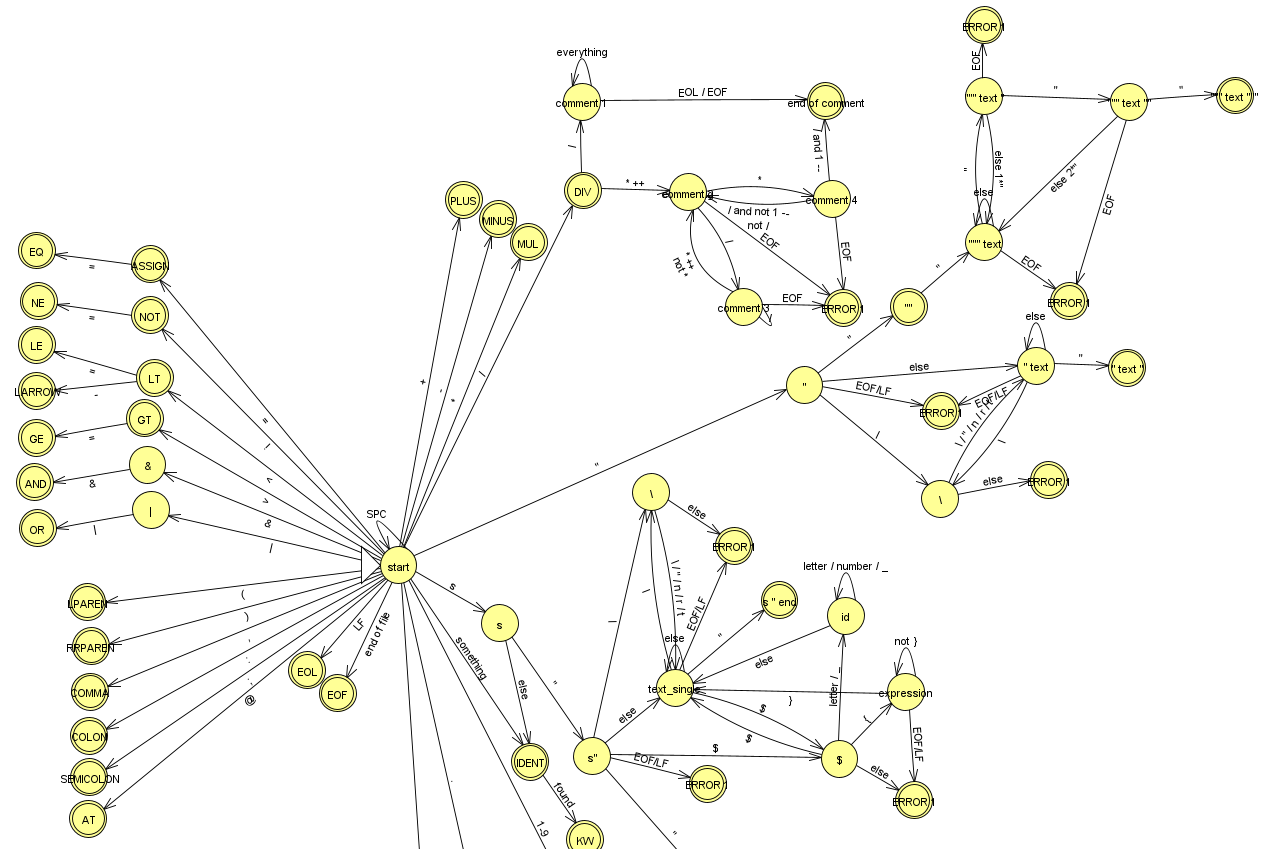
\includegraphics[width=\textwidth,height=0.45\textheight,keepaspectratio]{images/diagram_automatu_1.png}
    \caption{Konečný automat skenera 1. časť (operátory, komentáre, jednoriadkové reťazce a interpolácia)}
    \label{fig:diagram_automatu_1}
\end{figure}

\clearpage

\noindent
\begin{minipage}{\textwidth}
    \centering
    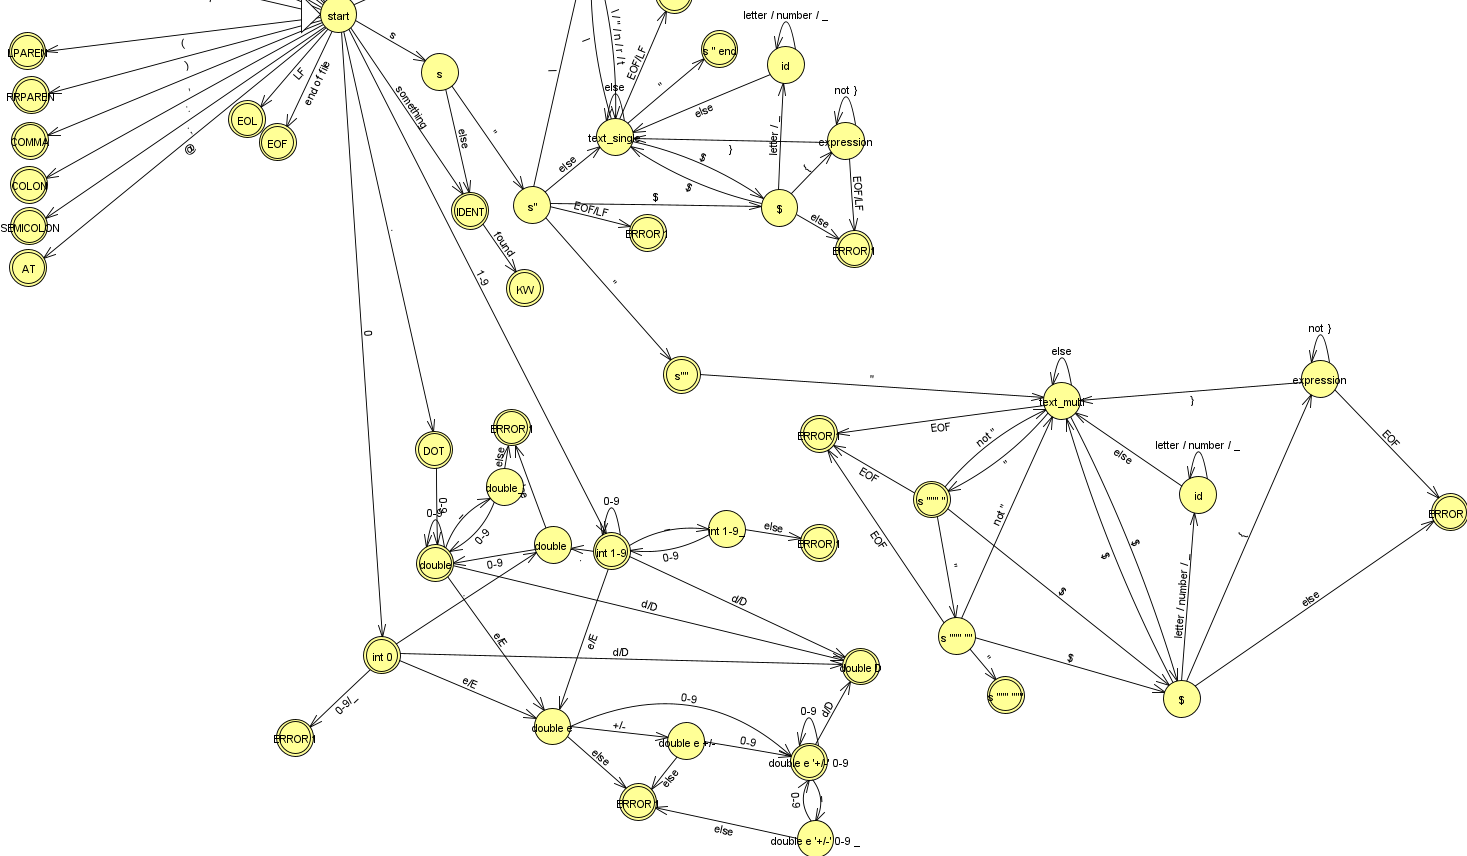
\includegraphics[width=\textwidth,height=0.45\textheight,keepaspectratio]{images/diagram_automatu_2.png}
    \captionof{figure}{Konečný automat skenera 2. časť (číselné literály a viacriadková interpolácia)}
    \label{fig:diagram_automatu_2}
\end{minipage}
\vspace{1em}

\section{Syntaktická analýza a LL(1) gramatika}

\subsection{Princíp}
Syntaktická analýza je založená na rekurzívnom zostupe podľa LL(1) gramatiky uvedenej nižšie (modul \texttt{parser.c}). Každý neterminál je implementovaný jednou funkciou, ktorá podľa aktuálneho tokenu vyberie pravidlo, a tokeny sa spotrebúvajú funkciou \texttt{compare\_token}. Tokeny parser neberie priamo zo skenera, ale z poľa, do ktorého ich pri inicializácii načíta všetky. Výrazy sa nespracúvajú rekurzívnym zostupom, ale samostatným precedenčným analyzátorom (modul \texttt{expr.c}, podsekcia \ref{sec:expr}), ktorý parser volá všade, kde gramatika obsahuje neterminál $\langle\text{EXP}\rangle$.

Parser nielen overuje syntax, ale súčasne \textbf{buduje abstraktný syntaktický strom} (\texttt{ast.h}) a vykonáva sémantické kontroly (kapitola o sémantickej analýze). Každá funkcia neterminálu vracia ukazovateľ na vytvorený uzol cez výstupný parameter a vlastníctvo uzla prechádza na volajúceho. Pri chybe funkcia uvoľní všetko, čo si dovtedy alokovala, takže sa pri žiadnom chybovom výstupe neuniká pamäť.

\subsection{Abstraktný syntaktický strom}
Koreňom stromu je uzol \texttt{NODE\_PROGRAM} so zoznamom funkcií a rozšírení (\texttt{extension}). Uzly sa delia na:
\begin{itemize}
    \item \textbf{definície:} \texttt{NODE\_FUNC\_DEF}, \texttt{NODE\_EXTENSION}, \texttt{NODE\_PARAM}, \texttt{NODE\_BLOCK},
    \item \textbf{príkazy:} \texttt{NODE\_VAL\_DEF}, \texttt{NODE\_VAR\_DEF}, \texttt{NODE\_ASSIGN}, \texttt{NODE\_IF\_STMT}, \texttt{NODE\_WHILE}, \texttt{NODE\_FOR}, \texttt{NODE\_RETURN}, \texttt{NODE\_EXPR\_STMT},
    \item \textbf{výrazy:} literály, \texttt{NODE\_ID}, \texttt{NODE\_UNARY\_OP}, \texttt{NODE\_BINARY\_OP}, \texttt{NODE\_CALL}, \texttt{NODE\_MEMBER}, \texttt{NODE\_ISTRING} a \texttt{NODE\_IF\_EXPR}.
\end{itemize}
Každý uzol nesie dátový typ (\texttt{DataType}) určený pri jeho vytvorení a pozíciu v zdrojovom kóde. Funkcie a volania s viacerými zoznamami parametrov (\texttt{f(a)(b, c)}) ukladajú parametre a argumenty ``naplocho'' spolu s poľom \texttt{list\_sizes}, ktoré hovorí, koľko z nich patrí do ktorých zátvoriek. Telo funkcie zapísané jedným výrazom sa uloží ako blok s jediným uzlom \texttt{NODE\_RETURN}.

\subsection{Predbežný prechod a dopredné volania}
Aby sa dala funkcia volať pred svojou definíciou, prejde parser po načítaní tokenov celé pole ešte raz (funkcia \texttt{prepass}). Sleduje pritom odsadenie a hľadá kľúčové slovo \texttt{def} na najvyššej úrovni a v telách rozšírení. Z každej hlavičky prečíta názov, zoznamy parametrov a prípadný návratový typ a zaregistruje ju v globálnej tabuľke symbolov spolu s pozíciou definície v poli tokenov. Hlavičku, ktorej nerozumie, preskočí, a chybu ohlási až samotný parser, keď na ňu dôjde.

Samotné parsovanie ide potom ako predtým rekurzívnym zostupom. Pri dosiahnutí \texttt{def} už existujúci symbol iba doplní, a ak je už označený ako definovaný, ide o redefiníciu. Návratový typ, ktorý nie je uvedený, sa odvodí z tela funkcie. Ak ho však potrebuje volanie skôr, než sa k telu dostane hlavný prechod, funkcia \texttt{resolve\_function} telo naparsuje vopred (\texttt{parse\_ahead}): uloží stav parsera, presunie sa na tokeny danej definície, vytvorí jej uzol a stav vráti späť. Hotový uzol sa zapamätá a keď hlavný prechod na túto definíciu príde, uzol len prevezme a tokeny preskočí. Poradie funkcií v AST tak zostáva rovnaké ako v zdrojovom texte. Ak sa funkcia bez uvedeného typu volá z vlastného tela (priamo alebo cez inú funkciu), jej typ ešte nie je známy a ide o chybu 6.

\subsection{Rozsahy platnosti}
Parser udržiava zreťazené tabuľky symbolov (\texttt{current\_scope}). Nový rozsah vzniká pre telo funkcie (spolu s parametrami), každý odsadený blok, jednoriadkový príkaz vo vetve \texttt{if}/\texttt{else} a v tele cyklu a pre cyklus \texttt{for} (riadiaca premenná je viditeľná iba v~strážach a tele). Premenná vzniká v tabuľke až po spracovaní svojho inicializačného výrazu, takže \texttt{val x = x + 1} sa správne odmietne ako použitie nedefinovaného identifikátora.

\subsection{LL(1) gramatika}
\small
\noindent
\begin{longtable}{p{0.5cm} p{3.0cm} p{6.2cm} p{3.8cm}}
\toprule
\textbf{Č.} & \textbf{Neterminál} & \textbf{Pravidlo (pravá strana)} & \textbf{Stručný popis} \\
\midrule
\endhead

\bottomrule
\endfoot

1 & $\langle\text{PROLOG}\rangle$ & $\rightarrow$ import id . * EOL $\langle\text{F\_LIST}\rangle$ EOF & Začiatok programu; identifikátor musí byť \texttt{ifj26}. \\
2 & $\langle\text{F\_LIST}\rangle$ & $\rightarrow$ $\langle\text{F\_DEF}\rangle$ $\langle\text{F\_LIST}\rangle$ & Ďalšia definícia funkcie. \\
3 & $\langle\text{F\_LIST}\rangle$ & $\rightarrow$ $\langle\text{EXTENSION}\rangle$ $\langle\text{F\_LIST}\rangle$ & Ďalšie rozšírenie typu. \\
4 & $\langle\text{F\_LIST}\rangle$ & $\rightarrow$ $\varepsilon$ & Koniec zoznamu definícií. \\
5 & $\langle\text{F\_DEF}\rangle$ & $\rightarrow$ $\langle\text{ANNOTATION}\rangle$ def id $\langle\text{PARAM\_LISTS}\rangle$ $\langle\text{D\_TYPE}\rangle$ = $\langle\text{F\_BODY\_END}\rangle$ & Definícia funkcie s voliteľnou anotáciou. \\
6 & $\langle\text{PARAM\_LISTS}\rangle$ & $\rightarrow$ ( $\langle\text{PARAMETER}\rangle$ ) $\langle\text{PARAM\_LISTS}\rangle$ & Zoznam parametrov; môže ich byť viac (currying). \\
7 & $\langle\text{PARAM\_LISTS}\rangle$ & $\rightarrow$ $\varepsilon$ & Koniec zoznamov parametrov. \\
8 & $\langle\text{F\_BODY\_END}\rangle$ & $\rightarrow$ EOL* INDENT $\langle\text{F\_BODY}\rangle$ DEDENT & Viacriadkové telo funkcie. \\
9 & $\langle\text{F\_BODY\_END}\rangle$ & $\rightarrow$ $\langle\text{EXP}\rangle$ EOL & Telo tvorené jedným výrazom (implicitný \texttt{return}). \\
10 & $\langle\text{ANNOTATION}\rangle$ & $\rightarrow$ @ main $\langle\text{NEW\_LINE}\rangle$ & Označenie funkcie \texttt{@main}. \\
11 & $\langle\text{ANNOTATION}\rangle$ & $\rightarrow$ $\varepsilon$ & Funkcia bez anotácie. \\
12 & $\langle\text{NEW\_LINE}\rangle$ & $\rightarrow$ EOL & Nový riadok za anotáciou. \\
13 & $\langle\text{NEW\_LINE}\rangle$ & $\rightarrow$ $\varepsilon$ & Bez nového riadku. \\
14 & $\langle\text{EXTENSION}\rangle$ & $\rightarrow$ extension ( id : $\langle\text{TYPE}\rangle$ ) EOL INDENT $\langle\text{E\_BODY}\rangle$ DEDENT & Rozšírenie typu o metódy; \texttt{id} je prijímač. \\
15 & $\langle\text{E\_BODY}\rangle$ & $\rightarrow$ def id $\langle\text{PARAM\_LISTS}\rangle$ $\langle\text{D\_TYPE}\rangle$ = $\langle\text{F\_BODY\_END}\rangle$ $\langle\text{EB\_NEXT}\rangle$ & Metóda rozšírenia. \\
16 & $\langle\text{EB\_NEXT}\rangle$ & $\rightarrow$ $\langle\text{E\_BODY}\rangle$ & Ďalšia metóda. \\
17 & $\langle\text{EB\_NEXT}\rangle$ & $\rightarrow$ $\varepsilon$ & Koniec metód. \\
18 & $\langle\text{D\_TYPE}\rangle$ & $\rightarrow$ : $\langle\text{TYPE}\rangle$ & Explicitný typ. \\
19 & $\langle\text{D\_TYPE}\rangle$ & $\rightarrow$ $\varepsilon$ & Typ nie je uvedený (odvodí sa). \\
20--24 & $\langle\text{TYPE}\rangle$ & $\rightarrow$ Int $\mid$ Double $\mid$ String $\mid$ Unit $\mid$ Boolean & Dátové typy. \\
25 & $\langle\text{PARAMETER}\rangle$ & $\rightarrow$ id : $\langle\text{TYPE}\rangle$ $\langle\text{PARAM\_NEXT}\rangle$ & Prvý parameter. \\
26 & $\langle\text{PARAMETER}\rangle$ & $\rightarrow$ $\varepsilon$ & Prázdny zoznam parametrov. \\
27 & $\langle\text{PARAM\_NEXT}\rangle$ & $\rightarrow$ , $\langle\text{PARAM\_TAIL}\rangle$ & Pokračovanie zoznamu. \\
28 & $\langle\text{PARAM\_NEXT}\rangle$ & $\rightarrow$ $\varepsilon$ & Koniec zoznamu. \\
29 & $\langle\text{PARAM\_TAIL}\rangle$ & $\rightarrow$ id : $\langle\text{TYPE}\rangle$ $\langle\text{PARAM\_NEXT}\rangle$ & Ďalší parameter. \\
30 & $\langle\text{PARAM\_TAIL}\rangle$ & $\rightarrow$ $\varepsilon$ & Koniec zoznamu (koncová čiarka). \\
31 & $\langle\text{F\_BODY}\rangle$ & $\rightarrow$ $\langle\text{STMT}\rangle$ $\langle\text{STMT\_NEXT}\rangle$ & Telo bloku. \\
32 & $\langle\text{STMT\_NEXT}\rangle$ & $\rightarrow$ EOL $\langle\text{STMT}\rangle$ $\langle\text{STMT\_NEXT}\rangle$ & Príkazy oddelené koncom riadku. \\
33 & $\langle\text{STMT\_NEXT}\rangle$ & $\rightarrow$ ; $\langle\text{STMT}\rangle$ $\langle\text{STMT\_NEXT}\rangle$ & Príkazy oddelené bodkočiarkou. \\
34 & $\langle\text{STMT\_NEXT}\rangle$ & $\rightarrow$ $\varepsilon$ & Koniec postupnosti príkazov; príkaz smie nasledovať priamo za blokom bez oddeľovača. \\
35 & $\langle\text{STMT}\rangle$ & $\rightarrow$ val id $\langle\text{D\_TYPE}\rangle$ = $\langle\text{EXP}\rangle$ & Nemenná premenná. \\
36 & $\langle\text{STMT}\rangle$ & $\rightarrow$ var id $\langle\text{D\_TYPE}\rangle$ = $\langle\text{EXP}\rangle$ & Menná premenná. \\
37 & $\langle\text{STMT}\rangle$ & $\rightarrow$ while $\langle\text{EXP}\rangle$ do EOL INDENT $\langle\text{F\_BODY}\rangle$ DEDENT & Cyklus \texttt{while}. \\
38 & $\langle\text{STMT}\rangle$ & $\rightarrow$ return $\langle\text{RET\_VAL}\rangle$ & Návrat z funkcie. \\
39 & $\langle\text{STMT}\rangle$ & $\rightarrow$ $\langle\text{EXP}\rangle$ & Výraz ako príkaz (napr. volanie funkcie). \\
40 & $\langle\text{STMT}\rangle$ & $\rightarrow$ $\langle\text{EXP}\rangle$ = $\langle\text{EXP}\rangle$ & Priradenie; ľavá strana musí byť identifikátor. \\
41 & $\langle\text{RET\_VAL}\rangle$ & $\rightarrow$ $\langle\text{EXP}\rangle$ & Návrat s hodnotou. \\
42 & $\langle\text{RET\_VAL}\rangle$ & $\rightarrow$ $\varepsilon$ & Návrat bez hodnoty. \\
48 & $\langle\text{STMT}\rangle$ & $\rightarrow$ $\langle\text{IF\_STMT}\rangle$ & Podmienený príkaz. \\
49 & $\langle\text{IF\_STMT}\rangle$ & $\rightarrow$ if $\langle\text{EXP}\rangle$ [then] ( EOL INDENT $\langle\text{F\_BODY}\rangle$ DEDENT $\mid$ $\langle\text{STMT}\rangle$ ) $\langle\text{IF\_NEXT}\rangle$ & Vetva \texttt{then} ako blok alebo jeden príkaz. \\
50 & $\langle\text{IF\_NEXT}\rangle$ & $\rightarrow$ else $\langle\text{ELSE\_NEXT}\rangle$ & Vetva \texttt{else}. \\
51 & $\langle\text{IF\_NEXT}\rangle$ & $\rightarrow$ $\varepsilon$ & Bez \texttt{else}. \\
52 & $\langle\text{ELSE\_NEXT}\rangle$ & $\rightarrow$ $\langle\text{IF\_STMT}\rangle$ & Reťazenie \texttt{else if}. \\
53 & $\langle\text{ELSE\_NEXT}\rangle$ & $\rightarrow$ EOL INDENT $\langle\text{F\_BODY}\rangle$ DEDENT $\mid$ $\langle\text{STMT}\rangle$ & Blok alebo jeden príkaz. \\
54 & $\langle\text{IF\_CONTROL}\rangle$ & $\rightarrow$ if $\langle\text{EXP}\rangle$ [then] $\langle\text{IF\_CTRL\_NEXT}\rangle$ else $\langle\text{IF\_CTRL\_NEXT}\rangle$ & \texttt{if} ako výraz; \texttt{else} je povinný. \\
55 & $\langle\text{IF\_CTRL\_NEXT}\rangle$ & $\rightarrow$ $\langle\text{EXP}\rangle$ & Vetva tvorená výrazom. \\
56 & $\langle\text{IF\_CTRL\_NEXT}\rangle$ & $\rightarrow$ EOL INDENT $\langle\text{F\_BODY}\rangle$ DEDENT & Vetva tvorená blokom. \\
57 & $\langle\text{STMT}\rangle$ & $\rightarrow$ for $\langle\text{FOR\_CONTENT}\rangle$ & Cyklus \texttt{for}. \\
59 & $\langle\text{FOR\_CONTENT}\rangle$ & $\rightarrow$ $\langle\text{GENERATOR}\rangle$ $\langle\text{OPT\_GUARDS}\rangle$ do $\langle\text{FOR\_BODY}\rangle$ & Jednoriadková hlavička. \\
60 & $\langle\text{FOR\_CONTENT}\rangle$ & $\rightarrow$ EOL INDENT $\langle\text{GENERATOR}\rangle$ $\langle\text{EOL\_GUARDS}\rangle$ DEDENT do $\langle\text{FOR\_BODY}\rangle$ & Viacriadková hlavička. \\
61 & $\langle\text{GENERATOR}\rangle$ & $\rightarrow$ id <- $\langle\text{EXP}\rangle$ $\langle\text{RANGE}\rangle$ $\langle\text{EXP}\rangle$ $\langle\text{OPT\_STEP}\rangle$ & Generátor hodnôt. \\
62, 63 & $\langle\text{RANGE}\rangle$ & $\rightarrow$ to $\mid$ until & Horná hranica vrátane / bez nej. \\
64 & $\langle\text{OPT\_STEP}\rangle$ & $\rightarrow$ by $\langle\text{EXP}\rangle$ & Krok. \\
65 & $\langle\text{OPT\_STEP}\rangle$ & $\rightarrow$ $\varepsilon$ & Bez kroku. \\
66 & $\langle\text{OPT\_GUARDS}\rangle$ & $\rightarrow$ if $\langle\text{EXP}\rangle$ $\langle\text{OPT\_GUARDS}\rangle$ & Stráž cyklu. \\
67 & $\langle\text{OPT\_GUARDS}\rangle$ & $\rightarrow$ $\varepsilon$ & Bez stráží. \\
68 & $\langle\text{EOL\_GUARDS}\rangle$ & $\rightarrow$ EOL if $\langle\text{EXP}\rangle$ $\langle\text{EOL\_GUARDS}\rangle$ & Stráž na samostatnom riadku. \\
69 & $\langle\text{EOL\_GUARDS}\rangle$ & $\rightarrow$ $\varepsilon$ & Bez ďalších stráží. \\
70 & $\langle\text{FOR\_BODY}\rangle$ & $\rightarrow$ $\langle\text{STMT}\rangle$ & Telo cyklu jedným príkazom. \\
71 & $\langle\text{FOR\_BODY}\rangle$ & $\rightarrow$ EOL INDENT $\langle\text{F\_BODY}\rangle$ DEDENT & Telo cyklu blokom. \\
\end{longtable}
\normalsize

\noindent Čísla pravidiel zodpovedajú komentárom v zdrojovom kóde \texttt{parser.c}. Pravidlá 43--47 pôvodnej verzie (neterminály \texttt{VAL}, \texttt{DEC}, \texttt{ARG}, \texttt{TERM}) zanikli, pretože ich nahradil precedenčný analyzátor výrazov, ktorý spracúva aj volania funkcií.

\subsection{Spracovanie výrazov (precedenčná syntaktická analýza)}
\label{sec:expr}
Výrazy spracúva modul \texttt{expr.c} pomocou zdola nahor riadeného precedenčného analyzátora so zásobníkom a precedenčnou tabuľkou. Zásobník obsahuje terminály (operátory, zátvorky, koncová značka \$) a neterminály $E$, ku ktorým je pripojený podstrom AST a jeho typ.

\begin{table}[!ht]
\centering
\small
\begin{tabular}{l|ccccccccccc}
 & \texttt{!} & $-_u$ & $*\;/$ & $+\;-$ & rel & $=\;\neq$ & \&\& & $\mid\mid$ & ( & ) & \$ \\
\hline
\texttt{!} & $<$ & $<$ & $>$ & $>$ & $>$ & $>$ & $>$ & $>$ & $<$ & $>$ & $>$ \\
$-_u$ & $<$ & $<$ & $>$ & $>$ & $>$ & $>$ & $>$ & $>$ & $<$ & $>$ & $>$ \\
$*\;/$ & $<$ & $<$ & $>$ & $>$ & $>$ & $>$ & $>$ & $>$ & $<$ & $>$ & $>$ \\
$+\;-$ & $<$ & $<$ & $<$ & $>$ & $>$ & $>$ & $>$ & $>$ & $<$ & $>$ & $>$ \\
rel & $<$ & $<$ & $<$ & $<$ & -- & $>$ & $>$ & $>$ & $<$ & $>$ & $>$ \\
$=\;\neq$ & $<$ & $<$ & $<$ & $<$ & $<$ & -- & $>$ & $>$ & $<$ & $>$ & $>$ \\
\&\& & $<$ & $<$ & $<$ & $<$ & $<$ & $<$ & $>$ & $>$ & $<$ & $>$ & $>$ \\
$\mid\mid$ & $<$ & $<$ & $<$ & $<$ & $<$ & $<$ & $<$ & $>$ & $<$ & $>$ & $>$ \\
( & $<$ & $<$ & $<$ & $<$ & $<$ & $<$ & $<$ & $<$ & $<$ & $=$ & -- \\
) & -- & -- & -- & -- & -- & -- & -- & -- & -- & -- & -- \\
\$ & $<$ & $<$ & $<$ & $<$ & $<$ & $<$ & $<$ & $<$ & $<$ & -- & acc \\
\end{tabular}
\caption{Precedenčná tabuľka tak, ako je v poli \texttt{PREC} v \texttt{expr.c} (riadok = terminál na vrchole zásobníka, stĺpec = vstupný terminál; rel = \texttt{< <= > >=}). Značka $<$ je posun, $>$ redukcia, $=$ spojenie zátvoriek, \texttt{--} chyba a \emph{acc} koniec výrazu.}
\end{table}

Priorita od najvyššej: unárne \texttt{!} a \texttt{-}, \texttt{*} \texttt{/}, \texttt{+} \texttt{-}, relačné operátory, \texttt{==} \texttt{!=}, \texttt{\&\&}, \texttt{||}. Operátory \texttt{+ - * /}, \texttt{\&\&} a \texttt{||} sú ľavo asociatívne. Relačné operátory (\texttt{< <= > >=}) a operátory rovnosti (\texttt{== !=}) asociatívne nie sú: v tabuľke je pre dvojicu rel--rel a rovnosť--rovnosť chyba, takže napríklad \texttt{a < b < c} je syntaktická chyba (kód 2). Ďalšie vlastnosti:
\begin{itemize}
    \item \textbf{Unárne a binárne mínus} sa rozlišujú podľa predchádzajúceho symbolu: ak bol predtým operand, ide o binárny operátor, inak o unárny.
    \item \textbf{Operandy} (literály, identifikátory, volania funkcií, \texttt{if} výraz a interpolované reťazce) sa spracujú rekurzívnymi pomocnými funkciami a uložia sa na zásobník ako neterminál $E$. Identifikátor funkcie sa spracuje ako volanie vrátane viacerých zoznamov argumentov \texttt{f(a)(b, c)}.
    \item \textbf{Prístup k členu} \texttt{x.meno} a \texttt{x.meno(args)} sa viaže silnejšie ako každý operátor. Hľadá sa v tomto poradí: metóda rozšírenia pre typ prijímača, funkcia s daným menom, ktorá berie prijímač ako prvý argument, a nakoniec vstavaný člen \texttt{toString}, \texttt{toInt}, \texttt{floor} alebo \texttt{length} (iba bez zátvoriek a len na vhodnom type).
    \item \textbf{Prázdne zátvorky} \texttt{()} tvoria hodnotu typu \texttt{Unit}.
    \item \textbf{Koniec výrazu} sa rozpozná na prvom tokene, ktorý ho nemôže predĺžiť (EOL, \texttt{then}, \texttt{do}, čiarka, nepárová \texttt{)} a pod.); analyzátor ho nespotrebuje.
    \item Pri každej redukcii $E \rightarrow E\ op\ E$ resp. $E \rightarrow op\ E$ sa kontrolujú typy operandov, určí sa typ výsledku a vytvorí sa uzol \texttt{NODE\_BINARY\_OP} resp. \texttt{NODE\_UNARY\_OP}.
\end{itemize}

\medskip
\noindent Samotný analyzátor funguje takto. Vstupným bodom \texttt{expr.c} je funkcia \texttt{parse\_expr}, ktorá pracuje so zásobníkom položiek \texttt{PItem}, kde každá položka je buď terminál (operátor, zátvorka, koncová značka), alebo neterminál $E$ s podstromom AST a jeho typom. Na začiatku je na zásobníku iba značka \$ a príznak \texttt{prev\_operand} hovorí, či bol posledný spracovaný symbol operand. V cykle sa pre aktuálny token urobí tento postup:
\begin{enumerate}
    \item Ak za operandom nasleduje bodka, zavolá sa \texttt{parse\_member} a operand na vrchole zásobníka sa nahradí uzlom \texttt{NODE\_MEMBER}.
    \item Ak token začína operand a predtým operand nebol, \texttt{parse\_primary} z neho vytvorí uzol a uloží ho na zásobník ako $E$. Podľa tokenu je to literál, interpolovaný reťazec (\texttt{interp\_string}), \texttt{if} výraz (\texttt{if\_control} z parsera) alebo identifikátor (\texttt{parse\_identifier}). Identifikátor premennej dostane typ zo symbolu. Pri funkcii sa načítajú zoznamy argumentov (\texttt{parse\_arg\_lists}), zavolá sa \texttt{resolve\_function}, \texttt{validate\_function\_call} skontroluje počet, štruktúru zoznamov a typy a vznikne uzol \texttt{NODE\_CALL}.
    \item Dvojica \texttt{()} sa nahradí hodnotou \texttt{Unit}.
    \item Inak sa token funkciou \texttt{classify} priradí k terminálu tabuľky. Token, ktorý výraz nemôže predĺžiť, sa zmení na koncovú značku \$.
    \item Potom sa porovná terminál najbližšie k vrcholu zásobníka so vstupným terminálom v tabuľke \texttt{PREC}. Pri posune sa vstupný terminál uloží a token sa spotrebuje. Pri redukcii sa zavolá \texttt{reduce}, ktorá odoberie operátor a operandy, skontroluje typy (\texttt{check\_unary}, \texttt{check\_binary}), vytvorí uzol a vloží späť výsledné $E$. Pri \texttt{=} sa zátvorky odstránia. Chyba v tabuľke ukončí analýzu kódom 2, nevhodné typy operandov pri redukcii kódom 6 a pri \emph{acc} je výraz hotový.
\end{enumerate}
Po prijatí musí na zásobníku zostať práve značka \$ a jediné $E$, ktorého uzol a typ sa vrátia volajúcemu. Zásobník vlastní všetky ešte nezačlenené podstromy, takže pri chybe v ktoromkoľvek kroku sa uvoľnia a nič neunikne.

\section{Sémantická analýza}

Sémantická analýza nie je samostatný prechod. Prebieha priebežne \textbf{počas syntaktickej analýzy}: parser pri spracovaní každého príkazu a pri každej redukcii vo výraze volá funkcie modulov \texttt{symtable}, \texttt{semantics} a \texttt{builtins}, takže už vytvorený AST je typovo anotovaný (každý uzol má vyplnené pole \texttt{type}).

\subsection{Tabuľka symbolov}
Tabuľka symbolov (\texttt{symtable.c}) je hašovacia tabuľka s reťazením synonym (funkcia DJB2, 101 záznamov). Každý rozsah platnosti má vlastnú tabuľku s odkazom na rodičovský rozsah, vyhľadávanie (\texttt{symtable\_lookup}) postupuje od aktuálneho rozsahu ku globálnemu, kým \texttt{symtable\_lookup\_local} hľadá iba v aktuálnom. Záznam obsahuje názov, druh (\texttt{SYMBOL\_VAR}, \texttt{SYMBOL\_VAL}, \texttt{SYMBOL\_FUNC}), dátový typ, príznak zmeniteľnosti a pre funkcie počet a typy parametrov. Vloženie už existujúceho názvu v tom istom rozsahu vráti \texttt{ERR\_SEMANTIC\_REDEFINITION}.

Funkcia sa do globálnej tabuľky vloží ešte pred spracovaním parametrov a tela. Jej signatúra (návratový typ, počet a typy parametrov) sa doplní hneď po prečítaní hlavičky, takže rekurzívne volania sa kontrolujú rovnako ako iné. Parametre sú uložené ako nezmeniteľné premenné.

\subsection{Vstavané funkcie}
Modul \texttt{builtins.c} pred spustením parsera zaregistruje do globálneho rozsahu funkcie jazyka IFJ26 s ich signatúrami: \texttt{readLine}, \texttt{readInt}, \texttt{readDouble}, \texttt{print}, \texttt{toStr}, \texttt{toInt}, \texttt{strLength}, \texttt{ord}, \texttt{chr} a \texttt{subStr}. Parameter typu \texttt{TYPE\_UNKNOWN} (pri \texttt{print} a \texttt{toStr}) zastupuje ``ľubovoľný typ''. Pamäť s typmi parametrov vlastní záznam a uvoľní sa v \texttt{symtable\_free}.

\subsection{Typový systém}
\begin{itemize}
    \item \textbf{Kompatibilita priradenia} (\texttt{is\_type\_compatible}): rovnaké typy, alebo \texttt{Int} do \texttt{Double}. Neznámy typ (\texttt{TYPE\_UNKNOWN}) je kompatibilný so všetkým, aby sa jedna chyba nešírila ďalej.
    \item \textbf{Aritmetika:} \texttt{+ - * /} nad \texttt{Int}/\texttt{Double}; ak je aspoň jeden operand \texttt{Double}, výsledok je \texttt{Double}. Operátor \texttt{+} je navyše definovaný nad dvojicou \texttt{String}.
    \item \textbf{Relačné operátory} \texttt{< <= > >=} sú definované nad číslami, výsledok je \texttt{Boolean}.
    \item \textbf{Rovnosť} \texttt{== !=} vyžaduje rovnaké (alebo obe číselné) typy, výsledok je \texttt{Boolean}.
    \item \textbf{Logické operátory} \texttt{\&\&}, \texttt{||} a \texttt{!} vyžadujú \texttt{Boolean}. Unárne \texttt{-} vyžaduje číslo.
    \item \textbf{Podmienky} v \texttt{if}, \texttt{while} a stráže cyklu \texttt{for} musia byť typu \texttt{Boolean}; hranice a krok cyklu \texttt{for} typu \texttt{Int}.
    \item \textbf{\texttt{if} ako výraz:} ak sa typy oboch vetiev líšia, ale obe sú číselné, výsledkom je \texttt{Double}; inak musia byť zhodné.
    \item \textbf{Odvodenie typu:} pri \texttt{val}/\texttt{var} bez uvedeného typu sa typ premennej odvodí z inicializačného výrazu.
\end{itemize}

\subsection{Kontroly a chybové kódy}
\begin{longtable}{p{0.8cm} p{6.3cm} p{7.5cm}}
\toprule
\textbf{Kód} & \textbf{Konštanta} & \textbf{Kedy nastane} \\
\midrule
\endhead
3 & \texttt{ERR\_SEMANTIC\_UNDEFINED} & použitie nedefinovanej premennej alebo funkcie; chýbajúca funkcia s anotáciou \texttt{@main} \\
4 & \texttt{ERR\_SEMANTIC\_REDEFINITION} & opätovná definícia funkcie alebo premennej v tom istom rozsahu \\
5 & \texttt{ERR\_SEMANTIC\_FUNCTION\_CALL} & zlý počet alebo typ argumentov volania; parametre pri funkcii \texttt{@main} \\
6 & \texttt{ERR\_SEMANTIC\_COMPATIBILITY} & nekompatibilný typ pri inicializácii, priradení, \texttt{return} alebo vetvách \texttt{if} výrazu \\
7 & \texttt{ERR\_SEMANTIC\_FORBIDDEN\_WRITING} & zápis do \texttt{val}, parametra funkcie alebo funkcie \\
8 & \texttt{ERR\_SEMANTIC\_TYPE} & nepovolené typy operandov operátora alebo nebooleovská podmienka \\
\bottomrule
\end{longtable}

Funkcia \texttt{validate\_function\_call} overí existenciu symbolu, že ide o funkciu, počet argumentov a kompatibilitu typu každého argumentu, a vráti návratový typ funkcie. Rovnakú kontrolu používa volanie cez bodku (\texttt{x.f(a)}), kde sa prijímač počíta ako prvý argument. Funkcia \texttt{check\_variable\_assignment} overí, že cieľ priradenia je zmeniteľná premenná (\texttt{var}). Pri návrate z funkcie (\texttt{return} aj jednovýrazové telo) sa typ výrazu porovnáva s deklarovaným návratovým typom.

\subsection{Známe obmedzenia}
Spracovanie je jednoprechodové, preto funkciu možno volať až po jej definícii v zdrojovom texte. Jazyk zatiaľ nevyužíva výsledky tejto analýzy na generovanie kódu (modul \texttt{codegen} nie je implementovaný).
\section{Generátor kódu}

\subsection{Architektura a princip generování}
Generování cílového kódu v jazyce \texttt{IFJcode26} zajišťuje modul \texttt{generator.c} (rozhraní v~\texttt{generator.h}). Inicializuje se funkcí \texttt{generator\_init(FILE~*out)} a spouští se nad hotovým, typově anotovaným stromem funkcí \texttt{generate\_program(AstNode~*node)}. Na konci funkce \texttt{generator\_cleanup} uvolní všechny interní tabulky a dynamicky alokované řetězce (spravované přes \texttt{pool\_add} / \texttt{pool\_printf}). Interní chyba alokace nebo neočekávaný stav uzlu nastaví \texttt{gen\_err = ERR\_INTERNAL\_COMPILER}.

Na začátku \texttt{generate\_program} generátor shromáždí všechny uživatelské funkce a metody rozšíření do pole \texttt{funcs} a dohledá funkci označenou \texttt{is\_main}. Následně vygeneruje hlavičku \texttt{.IFJcode26}, globální pomocné proměnné \texttt{GF@\_discard}, \texttt{GF@\_a}, \texttt{GF@\_b} a \texttt{GF@\_r}, zavolá \texttt{\$fn\_<main\_name>} a program ukončí instrukcí \texttt{EXIT int@0}. Poté připojí vestavěné funkce (\texttt{RUNTIME}) a postupně vygeneruje všechny funkce a metody rozšíření.

\subsection{Správa rámců a unikátních proměnných}
Každá funkce a metoda (\texttt{gen\_function}) začíná návěštím (\texttt{\$fn\_<jméno>} nebo \texttt{\$ext\_<Typ>\_<jméno>}), vytvoří si vlastní lokální rámec instrukcí \texttt{PUSHFRAME}, zadefinuje všechny své lokální proměnné a proměnné cyklů (\texttt{DEFVAR LF@...}) a před návratem rámec zruší pomocí \texttt{POPFRAME} a \texttt{RETURN}.

Aby se předešlo kolizi jmen při vnoření bloků a zastiňování proměnných:
\begin{itemize}
    \item \textbf{Deklarace v těle funkce:} Funkce \texttt{collect} projde tělo funkce před generováním instrukcí a pro každou \texttt{NODE\_VAL\_DEF} / \texttt{NODE\_VAR\_DEF} a cyklus \texttt{NODE\_FOR} (řídicí proměnná, \texttt{\_limit} a \texttt{\_step}) vytvoří unikátní název ve tvaru \texttt{<jméno>\%<číslo>} (tabulka \texttt{decls}). Všechny \texttt{DEFVAR} se tak vygenerují na začátku funkce a nikdy se neopakují ani v cyklech.
    \item \textbf{Viditelnost během průchodu:} Viditelné proměnné v aktuálním rozsahu se sledují na zásobníku \texttt{vars} se značkami bloků (\texttt{scope\_push} / \texttt{scope\_pop}). Parametry mají jména \texttt{\%p0}, \texttt{\%p1}, \dots\ (u metod rozšíření je \texttt{\%p0} příjemce).
\end{itemize}

\subsection{Výrazy, konverze a interpolované řetězce}
Vyhodnocování výrazů (\texttt{gen\_expr}) využívá datový zásobník interpreta (\texttt{PUSHS} / \texttt{POPS}) a probíhá v post-order pořadí:
\begin{itemize}
    \item \textbf{Literály a řetězce:} Celočíselné literály se ukládají jako \texttt{int@...}, desetinné jako \texttt{float@\%a}, logické jako \texttt{bool@true}/\texttt{bool@false} a \texttt{Unit} jako \texttt{nil@nil}. Řetězcové literály (\texttt{emit\_string\_const}) zapisují znaky s ASCII kódem $\le 32$, $35$ (\texttt{\#}), $92$ (\texttt{\textbackslash{}}) nebo $\ge 127$ jako escape sekvenci \texttt{\textbackslash{}xyz}.
    \item \textbf{Konverze \texttt{Int} $\rightarrow$ \texttt{Double}:} Jedinou implicitní konverzí je \texttt{Int} na \texttt{Double} (\texttt{gen\_coerce} přes \texttt{INT2FLOATS}). Při smíšených binárních operacích nad \texttt{Int} a \texttt{Double} (\texttt{gen\_binary}) se oba operandy převedou na \texttt{Double}; pokud jsou oba \texttt{Int}, celočíselné dělení používá \texttt{IDIVS} (u~\texttt{Double} \texttt{DIVS}).
    \item \textbf{Logické spojky a porovnání:} Operátory \texttt{\&\&} a \texttt{||} se vyhodnocují líně (\emph{short-circuit}) se skoky na \texttt{\$L<id>\_short}. Operátory $\le$ (\texttt{OP\_LE}) a $\ge$ (\texttt{OP\_GE}) se realizují jako negace \texttt{GTS}, resp. \texttt{LTS} pomocí \texttt{NOTS}, nerovnost \texttt{!=} jako \texttt{EQS} a \texttt{NOTS}.
    \item \textbf{Interpolované řetězce (\texttt{NODE\_ISTRING}):} Začínají vložením prázdného řetězce \texttt{string@}. Každá část se vyhodnotí, v případě jiného typu než \texttt{String} se zkonvertuje přes \texttt{\$ifj\_toStr} a připojí se instrukcí \texttt{CONCAT} přes globální proměnné \texttt{GF@\_a}, \texttt{GF@\_b} a \texttt{GF@\_r}.
\end{itemize}

\subsection{Volání funkcí a přístup ke členům}
Volání uživatelských funkcí, vestavěných funkcí (\texttt{\$ifj\_...}) i metod rozšíření (\texttt{gen\_invoke}) nejprve vyhodnotí příjemce (pokud jde o metodu nebo volání přes tečku) a všechny argumenty na datový zásobník s případnou konverzí na typ parametru. Poté se vytvoří nový rámec (\texttt{CREATEFRAME}), naplní se proměnné \texttt{TF@\%p0}, \texttt{TF@\%p1}, \dots\ v opačném pořadí od vrcholu zásobníku a zavolá se cílové návěští (\texttt{CALL}).

Funkce \texttt{gen\_member} řeší \texttt{x.jméno} a \texttt{x.jméno(args)} v tomto pořadí: nejprve hledá metodu rozšíření pro typ příjemce, poté vestavěné členy (\texttt{toString} $\rightarrow$ \texttt{\$ifj\_toStr}, \texttt{length} $\rightarrow$ \texttt{\$ifj\_strLength}, \texttt{toInt} $\rightarrow$ \texttt{\$ifj\_toInt}, \texttt{floor} $\rightarrow$ \texttt{\$ifj\_floor}) a nakonec obyčejnou funkci s příjemcem jako prvním argumentem. Návratová hodnota funkce zůstává na vrcholu datového zásobníku; pokud příkaz \texttt{NODE\_EXPR\_STMT} nebo funkce typu \texttt{Unit} hodnotu nepotřebuje, odebere se do \texttt{GF@\_discard}.

\subsection{Podmínky, cykly \texttt{while} a \texttt{for}}
Generátor přiděluje každému větvení nebo cyklu unikátní číselné ID (\texttt{new\_label}):
\begin{itemize}
    \item \textbf{Větvení (\texttt{NODE\_IF\_STMT}, \texttt{NODE\_IF\_EXPR}):} Vyhodnotí podmínku a při hodnotě \texttt{false} skočí na \texttt{\$L<id>\_else} (\texttt{gen\_jump\_if\_false}). U \texttt{NODE\_IF\_EXPR} se hodnota každé větve získá přes \texttt{gen\_value} (v bloku se vrátí hodnota posledního výrazu, jinak \texttt{nil@nil}) a přetypuje na cílový typ uzlu.
    \item \textbf{Cyklus \texttt{while} (\texttt{NODE\_WHILE}):} Na návěští \texttt{\$L<id>\_start} vyhodnotí podmínku, při \texttt{false} skočí na \texttt{\$L<id>\_end}, vykoná tělo a skočí zpět na \texttt{\$L<id>\_start}.
    \item \textbf{Cyklus \texttt{for} (\texttt{NODE\_FOR}):} Hranice \texttt{from}, \texttt{to} a případný krok \texttt{by} (jinak \texttt{int@1}) se vyhodnotí jednou před první iterací do proměnných v \texttt{LF}. Nulový krok ukončí program s chybovým kódem \texttt{40} (\texttt{EXIT int@40}). V každé iteraci (\texttt{\$L<id>\_test}) se otestuje hranice podle znaménka kroku a režimu \texttt{to} / \texttt{until}, v novém rozsahu se zpřístupní řídicí proměnná, postupně se vyhodnotí všechny stráže (\emph{guards}; při \texttt{false} se skočí na \texttt{\$L<id>\_next}), vykoná se tělo cyklu a na \texttt{\$L<id>\_next} se přičte krok.
\end{itemize}

\subsection{Runtime vestavěných funkcí}
Řetězec \texttt{RUNTIME} definuje instrukce \texttt{IFJcode26} pro vestavěné funkce jazyka IFJ26: \texttt{\$ifj\_print} (hodnotu \texttt{nil} vypisuje jako \texttt{()}), \texttt{\$ifj\_toStr} (převádí \texttt{int}, \texttt{float}, \texttt{bool}, \texttt{string} a \texttt{nil} $\rightarrow$ \texttt{()}), \texttt{\$ifj\_readLine}, \texttt{\$ifj\_readInt}, \texttt{\$ifj\_readDouble}, \texttt{\$ifj\_readBoolean} (při \texttt{nil}/EOF vracejí výchozí hodnoty \texttt{""}, \texttt{0}, \texttt{0.0}, resp. \texttt{false}), \texttt{\$ifj\_strLength}, \texttt{\$ifj\_ord} (mimo rozsah vrací \texttt{-1}), \texttt{\$ifj\_chr}, \texttt{\$ifj\_subStr} (neplatný rozsah končí \texttt{EXIT int@40}), \texttt{\$ifj\_toInt} a \texttt{\$ifj\_floor}.

\end{document}

\section{Prehľad modulov}
Kompletný zoznam zdrojových súborov prekladača:
\begin{itemize}
    \item \texttt{main.c} -- Vstupný bod. Inicializuje skener, globálnu tabuľku symbolov a vstavané funkcie, spustí parser, uvoľní všetky zdroje a vráti chybový kód prekladača.
    \item \texttt{scanner.c} / \texttt{scanner.h} / \texttt{indent\_stack.c} / \texttt{indent\_stack.h} / \texttt{string\_buffer.c} / \texttt{string\_buffer.h} / \texttt{token.h} -- Lexikálna analýza (konečný automat, zásobník odsadenia, dynamický reťazcový buffer, definícia tokenov).
    \item \texttt{parser.c} / \texttt{parser.h} -- Syntaktická analýza rekurzívnym zostupom (definície, príkazy, bloky, cykly) a tvorba AST; riadi rozsahy platnosti. Obsahuje aj pole načítaných tokenov a predbežný prechod, ktorý registruje hlavičky funkcií.
    \item \texttt{expr.c} / \texttt{expr.h} -- Precedenčná syntaktická analýza výrazov, tvorba uzlov výrazov, kontrola typov operátorov, volania funkcií, prístup k členom, interpolované reťazce a \texttt{if} výraz.
    \item \texttt{ast.c} / \texttt{ast.h} -- Abstraktný syntaktický strom: typy uzlov, konštruktory a rekurzívne uvoľnenie stromu.
    \item \texttt{symtable.c} / \texttt{symtable.h} -- Hašovacia tabuľka symbolov so zreťazenými rozsahmi platnosti.
    \item \texttt{semantics.c} / \texttt{semantics.h} -- Sémantické kontroly: kompatibilita typov, zmeniteľnosť premenných, overenie volania funkcie (počet, štruktúra zoznamov a typy argumentov).
    \item \texttt{builtins.c} / \texttt{builtins.h} -- Registrácia vstavaných funkcií jazyka IFJ26 do globálnej tabuľky symbolov.
    \item \texttt{generator.c} / \texttt{generator.h} -- Generovanie kódu IFJcode26 z hotového AST.
    \item \texttt{error.h} -- Zoznam chybových kódov prekladača.
\end{itemize}

\subsection{Závislosti modulov}
\begin{center}
\texttt{main} $\rightarrow$ \{ \texttt{scanner}, \texttt{parser}, \texttt{symtable}, \texttt{builtins}, \texttt{generator} \}; \quad \texttt{scanner} $\rightarrow$ \{ \texttt{indent\_stack}, \texttt{string\_buffer} \}; \quad \texttt{parser} $\rightarrow$ \{ \texttt{scanner}, \texttt{expr}, \texttt{semantics}, \texttt{ast}, \texttt{symtable} \}; \quad \texttt{generator} $\rightarrow$ \texttt{ast}; \quad \texttt{expr} $\rightarrow$ \{ \texttt{parser} (\texttt{compare\_token}, \texttt{if\_control}), \texttt{semantics}, \texttt{ast} \}; \quad \texttt{semantics} $\rightarrow$ \texttt{symtable}; \quad \texttt{builtins} $\rightarrow$ \texttt{symtable}.
\end{center}
\section{Využitie prostriedkov AI}
Počas vývoja sme umelú inteligenciu (Claude Sonet 5.5) používali iba ako pomocný nástroj.
\begin{itemize}
	\item \textbf{Spôsob použitia:} AI sme využívali na kontrolu nami napísaného kódu, ako pomoc pri hľadaní chýb a okrajových prípadov.
	\item \textbf{Overovanie:} Ak AI nás na niečo upozornilo, tak sme si to overili pomocou \texttt{Specifikace jazyků IFJ26 a IFJcode26}.
	\item \textbf{Obmedzenia:} AI nebolo využité na zakázané časti ako (tabuľky symbolov, LL gramatiky, automatu, precedenčnej tabuľky).
\end{itemize}

\section{Bibliografické citácie}
\begin{thebibliography}{9}
    \bibitem{ifj_lectures} Študijné materiály predmetu IFJ na FIT VUT v Brne.
\end{thebibliography}

\end{document}